\begin{figure}[t]
  \centering
  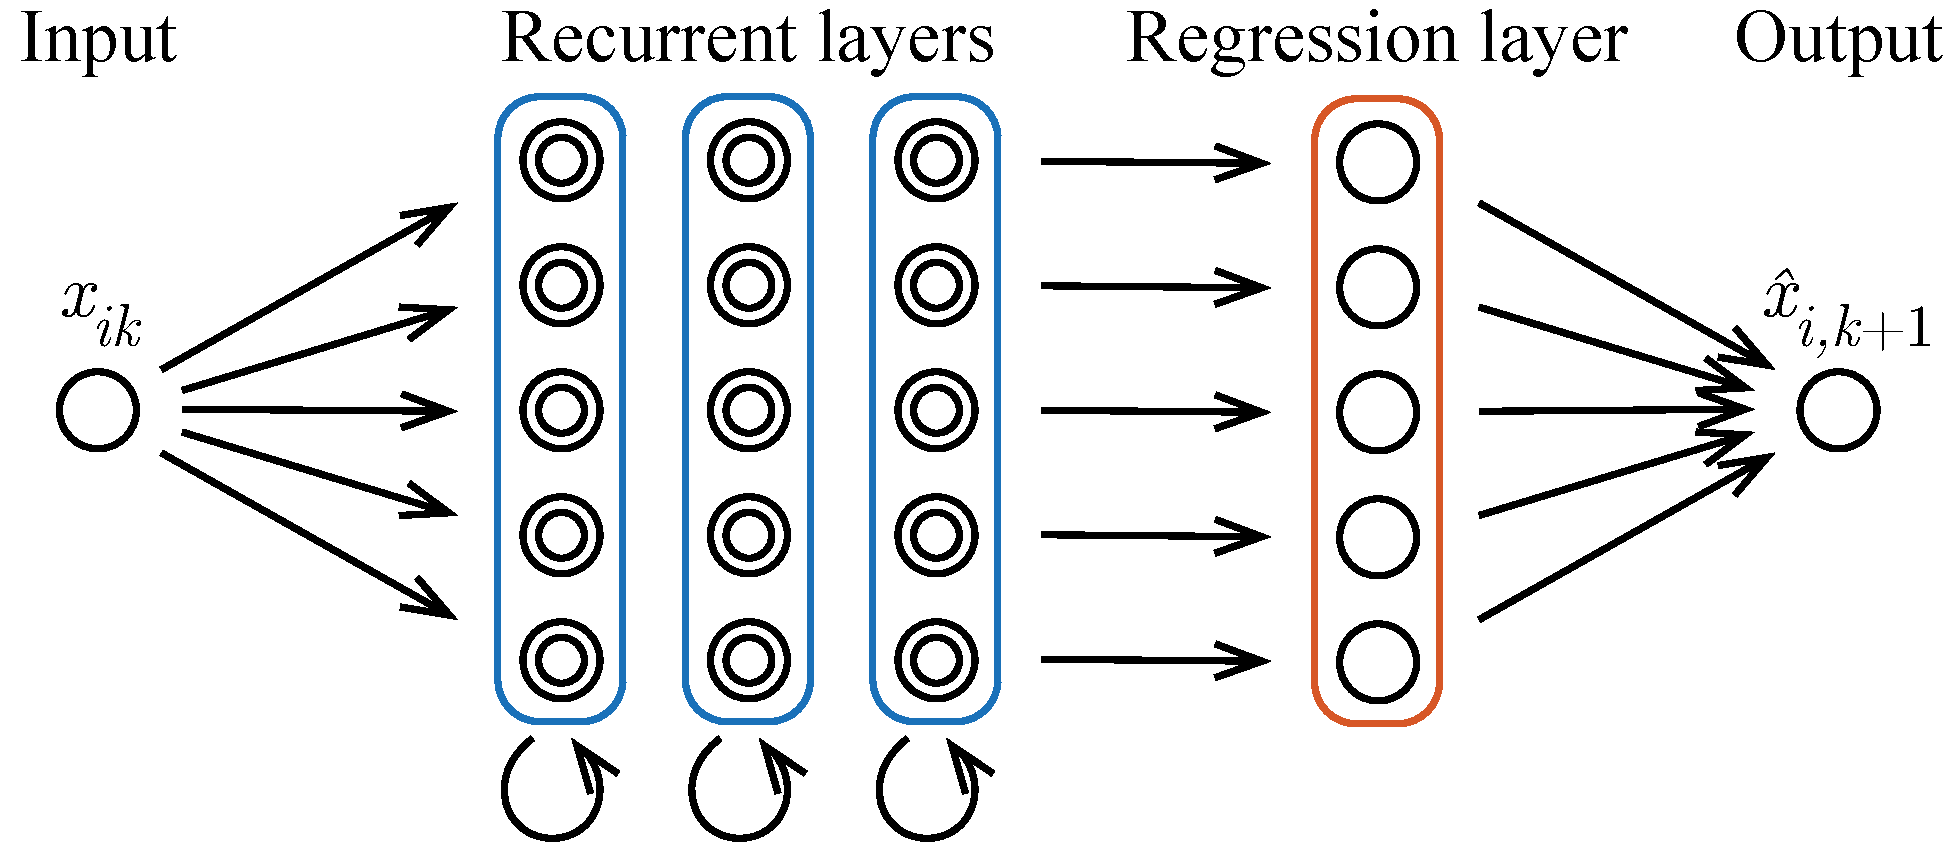
\includegraphics[width=1.0\columnwidth]{include/assets/figures/model.pdf}
  \caption{A schematic representation of our predictive model.}
  \vspace{-1.5em}
  \flab{model}
\end{figure}

As mentioned in \sref{introduction} and \sref{problem}, a part of our goal is to
assess the applicability of the latest advancements in neural networks
\cite{goodfellow2016} to modeling and prediction of fine-grained resource-usage
data. The architectures of neural networks are very diverse: one network can be
nothing like another. Since the data that we study are inherently sequential, it
is natural to found our model on the basis of recurrent neural networks
\cite{goodfellow2016}, which are specifically designed for such cases as ours.

A schematic representation of our model can be seen in \fref{model}; many of the
actual connections between the model's parts are simplified or not shown at all
in order to make the figure legible. In the following subsections, we shall
describe each part in detail; a number of important operational aspects of the
model will be covered in the next section, \sref{operation}.

\subsection{Input and Output}
The input to the model is a single $d$-dimensional data point, which can be seen
on the left-hand side of \fref{model}. Similarly, the output is a single
$d$-dimensional data point, which is depicted on the right-hand side of
\fref{model}. The input $x_{ik}$ is the value of the resource usage of an
individual task at step $k$, and the output $\hat{x}_{i,k + 1}$ is a
one-step-ahead prediction of the usage.

\subsection{Recurrent Layers} \slab{recurrent}
The core of the model is formed by a number of recurrent layers, which are
represented by a group of blue boxes in \fref{model}. The network can be made as
many layers deep as needed. Each layer, which is also referred to as a cell, is
composed of a number of units, which are the smallest processing elements. The
key characteristics of a unit are that it has memory, and that it has access to
its previous output, which makes it recurrent.

There are different types of units; each one defines how a unit lets data flow
through it and updates its memory. One notable type is called \up{LSTM}
\cite{hochreiter1997}, which stands for \emph{long short-term memory}. It has
been designed to overcome the problems of traditional recurrent networks---such
as vanishing gradient when training---and it is now one of the most widely used
types. The recurrent layers of our model are \up{LSTM} cells.

In addition, each cell is enhanced with a dropout mechanism \cite{zaremba2014}.
This mechanism gives control over the regularization of the model and is to
prevent potential overfitting \cite{hastie2009}.

\subsection{Regression Layer}
The output of the last cell is typically a large tensor, which is proportional
in size to the number of units in the cell. Each entry of such a tensor can be
considered as a feature that the network has extracted and activated in
accordance with the trace that is currently being fed into the model. The task
now is combine these features in order to produce a single prediction. To this
end, we mount a regression layer on top of the last cell, which is depicted by a
red box in \fref{model}. Unlike the recurrent layers described in
\sref{recurrent}, which features highly nonlinear transformations, this layer
performs an affine transformation.

To summarize, we have described a predictive model that is composed of a number
of \up{LSTM} cells and a linear regression layer. Due to its internal memory,
the model is capable of efficiently taking into account the entire past of the
resource-usage trace under consideration when making predictions. Let us now
discuss how the model is supposed to be used.
